\documentclass[12pt]{article}
\usepackage{{../preamble}}
\graphicspath{{pics}}
\begin{document}
% \maketitle
\chead{Problem Set 1}

%%%%%%%%%%%%%%%%%%%%%%%%%%%%%%%%%%%%%%%%%%%%%%%
%                  Definitions                %
%%%%%%%%%%%%%%%%%%%%%%%%%%%%%%%%%%%%%%%%%%%%%%%
%\includegraphics[width=\mywidth\textwidth]{}

% \begin{figure}[h!]
% \centering
% \input{pics/PS2/p7b}
% \caption{}
% \label{fig-}
% \end{figure}

% \begin{enumerate}[label=\alph*.]
%     \setcounter{enumi}{1}
%     \item 
% \end{enumerate}

%%%%%%%%%%%%%%%%%
%     Part a    %
%%%%%%%%%%%%%%%%%


%%%%%%%%%%%%%%%%%%%%%%%%%%%%%%%%%%%%%%%%%%%%%%%
%                Problem 1                    %
%%%%%%%%%%%%%%%%%%%%%%%%%%%%%%%%%%%%%%%%%%%%%%%
\def\xdot{\dot X} \def\ydot{\dot Y} \def\zdot{\dot Z}
\def\kdot{\dot k} \def\ddt{\frac{d}{dt}}
\section*{Problem 1}
\problem{Basic Properties of Growth Rates: Romer 1.1}{
    Use the fact that the growth rate of a variable
equals the time derivative of its log to show:
    \begin{enumerate}[label=(\alph*)]
    \item The growth rate of the product of two variables equals the sum of their growth rates. That is, if $Z(t)= X(t)Y(t)$, then $\zdot(t)/Z(t) = [\xdot(t)/X(t)] + [\ydot(t)/Y(t)]$.
    \end{enumerate} 
}

\begin{align*} 
    \intertext{Assuming $Z=XY$ and $X,Y$ are both univariate functions of $t$, then}
    \frac{\zdot}{Z} &= \ddt \ln Z \\
        &= \ddt \ln(XY) \\
        &= \ddt (\ln X + \ln Y) \\
        &= \ddt\ln X + \ddt\ln Y \\
        &= \frac{\xdot}{X} + \frac{\ydot}{Y}
\end{align*}



%%%%%%%%%%%%%%%%%
%     Part b    %
%%%%%%%%%%%%%%%%%
\newpage\problem{}{
    \begin{enumerate}[label=(\alph*)]
    \setcounter{enumi}{1}
    \item The growth rate of the ratio of two variables equals the difference of their growth rates. That is, if $Z(t)= X(t)/Y(t)$, then $\dot Z(t)/Z(t) = [\xdot(t)/X(t)]-[\ydot(t)/Y(t)]$.
    \end{enumerate} 
}

\begin{align*} 
    \intertext{Assuming $Z=X/Y$ and $X,Y$ are both univariate functions of $t$, then}
    \frac{\zdot}{Z} &= \ddt \ln Z \\
        &= \ddt \ln(X/Y) \\
        &= \ddt (\ln X - \ln Y) \\
        &= \ddt\ln X - \ddt\ln Y \\
        &= \frac{\xdot}{X} - \frac{\ydot}{Y}
\end{align*}


\newpage
%%%%%%%%%%%%%%%%%
%     Part c    %
%%%%%%%%%%%%%%%%%
\newpage\problem{}{
    \begin{enumerate}[label=(\alph*)]
    \setcounter{enumi}{2}
    \item If $Z(t) = \alpha X(t)^\alpha$, then $\zdot(t)/Z(t) = \alpha \xdot(t)/X(t)$.
    \end{enumerate} 
}

\begin{align*} 
    \intertext{Assuming $Z=\alpha X^\alpha$ and $X$ is a univariate function of $t$, then}
    \frac{\zdot}{Z} &= \ddt \ln Z \\
        &= \ddt \ln(\alpha X^\alpha) \\
        &= \ddt (\ln\alpha + \alpha\ln X) \\
        &= \ddt\ln\alpha + \alpha\ddt\ln X \\
        &= 0 + \alpha\frac{\xdot}{X}
\end{align*}












%%%%%%%%%%%%%%%%%%%%%%%%%%%%%%%%%%%%%%%%%%%%%%%
%                Problem 2                    %
%%%%%%%%%%%%%%%%%%%%%%%%%%%%%%%%%%%%%%%%%%%%%%%
\newpage
\section*{Problem 2}
\def\slope{\text{Slope}} 
\problem{Constant-Elasticity-of-Substitution Production Functions}{
    Consider the production function
    \begin{equation}
    Y = F(K,L) = A[aK^\phi + (1-a) L^\phi]^{1/\phi}
    \label{eq:F2}
    \end{equation}
    where $0<a<1$ and $\phi<1$.
    \vspace{1em}

    Recall that the elasticity of substitution between capital and labor is the curvature of the isoquants of the production function. The slope of an isoquant is
    \begin{equation*}
        \slope = \frac{\partial F(\cdot)/\partial K}{\partial F(\cdot)/\partial L}
    \end{equation*}

    The elasticity is then
    \begin{equation*}
    \left[
        \frac{\partial (\slope)}{\partial (L/K)}
        \frac{L/K}{\slope}
    \right]^{-1}
    \end{equation*}

    \begin{enumerate}[label=(\alph*)]
        \item Show that the elasticity of subtitution of the production function \eqref{eq:F2} is constant and equal to $1/(1-\phi)$.
    \end{enumerate} 
}

\def\dfdk{\frac{\partial F}{\partial K}}
\def\dfdl{\frac{\partial F}{\partial L}}
\begin{align*} 
    \intertext{First, let's find both partial derivatives of \eqref{eq:F2}}
    \dfdk &= A\frac{1}{\phi}[...]^{1/\phi-1}aK^{\phi-1} \\
    \dfdl &= A\frac{1}{\phi}[...]^{1/\phi-1}(1-a)L^{\phi-1}
\intertext{So, with some cancellation, the slope is then}
    \slope &= \dfrac{\frac{\partial F}{\partial K}}{\frac{\partial F}{\partial L}} \\
        &= \frac{a}{1-a}\left(\frac{K}{L}\right)^{\phi-1} \\
        &= \frac{a}{1-a}\left(\frac{L}{K}\right)^{1-\phi} 
\intertext{Then }
    \frac{\partial (\slope)}{\partial (L/K)}
    &= \frac{a}{1-a}(1-\phi)\left(\frac{L}{K}\right)^{-\phi} \\
    &= (1-\phi)\left(\frac{L}{K}\right)^{-1}\slope
\intertext{And finally, the elasticity of substitution between capital and labor is}
\left[
    \frac{\partial (\slope)}{\partial (L/K)}
    \frac{L/K}{\slope}
\right]^{-1}
    &= \left[
        (1-\phi)\left(\frac{L}{K}\right)^{-1}\slope
        \frac{L/K}{\slope}
        \right]^{-1}\\
    &= (1-\phi)^{-1}
\end{align*}



%%%%%%%%%%%%%%%%%
%     Part b    %
%%%%%%%%%%%%%%%%%
\problem{}{
    \begin{enumerate}[label=(\alph*)]
    \setcounter{enumi}{1}
    \item Show that when the elasticity of substitution approaches 1 ($\phi\to 0$), this production function approaches the Cobb-Douglas form $Y = (\text{constant})K^\alpha L^{1-\alpha}$.
    
    (Hint: You will need to use l’Hopital’s rule.)
    \end{enumerate} 
}
\def\plim{\lim\limits_{\phi\to 0}}
\def\ddp{\dfrac{\partial}{\partial \phi}}
\def\dgdp{\dfrac{\partial\gamma}{\partial \phi}}
\begin{align*} 
    \intertext{Because $\ln(\cdot)$ is monotone and we expect the output to always be positive, we just need to show that $\ln(F)$ is equal to the log form of a Cobb-Douglas in the limit:}
    \text{Let } \gamma &= aK^\phi + (1-a) L^\phi \\
    \text{Then } \dgdp &= aK^\phi\ln K + (1-a) L^\phi \ln L \\
    \text{and } \ln F &= \ln A + \frac{1}{\phi} \ln \gamma \\[1em]
    \plim\ln \frac{F}{A} &= 
        \dfrac{\plim\ddp\ln\gamma}{\plim\ddp\phi} \\[1em]
        &=\dfrac{\plim\dfrac{1}{\gamma}\ddp\gamma}{1} \\[1em]
        &=\plim\frac{aK^\phi\ln K + (1-a) L^\phi \ln L}{aK^\phi + (1-a) L^\phi} \\[1em]
        &=\frac{a\ln K + (1-a)\ln L}{a + 1 - a} \\[.5em]
        &=\ln [K^a L^{1-a}]
    \intertext{Which implies}
    \plim F &= A K^a L^{1-a}
\end{align*}



%%%%%%%%%%%%%%%%%
%     Part c    %
 %%%%%%%%%%%%%%%%% \newpage
\newpage
\def\invphi{\sfrac{1}{\phi}}
\problem{}{
    \begin{enumerate}[label=(\alph*)]
    \setcounter{enumi}{2}
    \item Divide through equation \eqref{eq:F2} by L and rewrite the production function in terms of output per person $y$ and capital per person $k$. Let’s refer to this production function as $y = f(k)$.
    \end{enumerate} 
}

\begin{align*} 
    y&= f(k) \\
    &= \frac{F}{L} \\
    &= A\left[ \frac{1}{L^\phi}\Big(aK^\phi + (1-a) L^\phi \Big) \right]^\invphi \\
    &= A[ak^\phi + (1-a)]^\invphi
\end{align*}



%%%%%%%%%%%%%%%%%
%     Part d    %
%%%%%%%%%%%%%%%%%
\newpage\problem{}{
    \begin{enumerate}[label=(\alph*)]
    \setcounter{enumi}{3}
    \item Derive expressions for $f'(k)$ and $f(k)/k$.
    \end{enumerate} 
}

\begin{align*} 
    \frac{f(k)}{k} &= \frac{A}{k}[ak^\phi + (1-a)]^\invphi \\
        &= A[a + (1-a)k^{-\phi}]^\invphi  \\[2em]
    f'(k) &= A\frac{1}{\phi}[ak^\phi + (1-a)]^{\invphi-1}a\phi k^{\phi-1} \\
        &= \frac{Aa[ak^\phi + (1-a)]^{\invphi-1}}{k^{1-\phi}} \\
        &= Aa[a + (1-a)k^{-\phi}]^{\invphi-1} \\[2em]
    \intertext{Note that}
    f'(k) &= A^\phi a\left(\frac{f(k)}{k}\right)^{1-\phi}
\end{align*}



%%%%%%%%%%%%%%%%%
%     Part e    %
%%%%%%%%%%%%%%%%%
\newpage\problem{}{
    \begin{enumerate}[label=(\alph*)]
    \setcounter{enumi}{4}
    \item Consider the case where capital and labor are gross substitutes ($0 < \phi < 1$). Does the production function satisfy the Inada conditions?
    \end{enumerate} 
}

\begin{align*} 
    \intertext{Assume $\phi\in(0,1)$. First consider the limit as $k\to 0$: }
    \lim_{k\to 0}f'(k) &= \lim_{k\to 0}\frac{Aa[ak^\phi + (1-a)]^{\invphi-1}}{k^{1-\phi}}  = \infty
    \intertext{so the first Inada conditions is met. Let's now consider the limit as $k\to\infty$. Using the relationship between $f'$ and $f/k$ from the last problem, we have:}
    \lim_{k\to\infty}f'(k) 
        &= \lim_{k\to\infty}A^\phi a\left(\frac{f(k)}{k}\right)^{1-\phi}\\
        &= A^\phi a\left(\lim_{k\to\infty}\frac{f(k)}{k}\right)^{1-\phi}\\[1em]
    \lim_{k\to\infty}\frac{f(k)}{k}
        &=  \lim_{k\to\infty} A[a + (1-a)k^{-\phi}]^\invphi \\
        &=   A[a + (1-a)\lim_{k\to\infty}k^{-\phi}]^\invphi \\
        &=   Aa^\invphi \\
        &\neq 0
    \intertext{And because $\phi\in(0,1)$,}
    \implies \lim_{k\to\infty}f'(k) &\neq 0
    \intertext{So this production function does not satisfy the Inada conditions.}
\end{align*}



%%%%%%%%%%%%%%%%%
%     Part f    %
%%%%%%%%%%%%%%%%%
\newpage\problem{}{
    \begin{enumerate}[label=(\alph*)]
    \setcounter{enumi}{5}
    \item Recall that
    \[\frac{\kdot}{k} = \frac{sf(k)}{k} - (n+\delta)\]
    where $s$ is the savings rate, $n$ is the population growth rate, and $\delta$ is the depreciation rate of capital.
    \vspace{1em}
    
    Can capital accumulation result in sustained growth in this economy given a constant savings rate?
    (Hint: Plot $sf(k)/k$ and $(n + \delta)$ as a function of $k$ on the same figure.)
    \end{enumerate} 
}

Note from the last problem that $\lim_{k\to\infty}\frac{sf(k)}{k} =sAa^\invphi>0$. So in the case where $n+\delta > sAa^\invphi$, the plot would look like

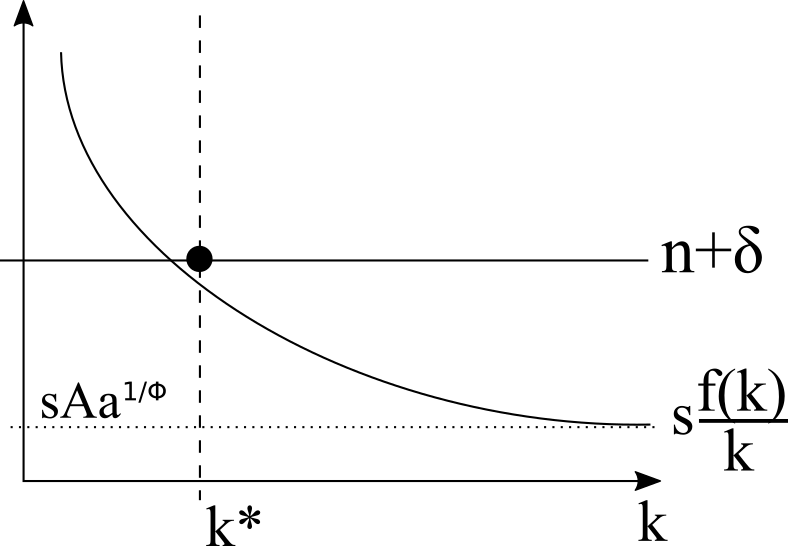
\includegraphics[width=0.5\textwidth]{2f-a}

We can see in the above picture that there is a $k^*$ where $n+\delta$ meets $\frac{sf(k)}{k}$, indicating that there is a steady state in capital per unit of effective labor and that capital accumulation alone cannot lead to sustained growth. If we consider the case where $n+\delta < sAa^\invphi$, the plot would look like this:

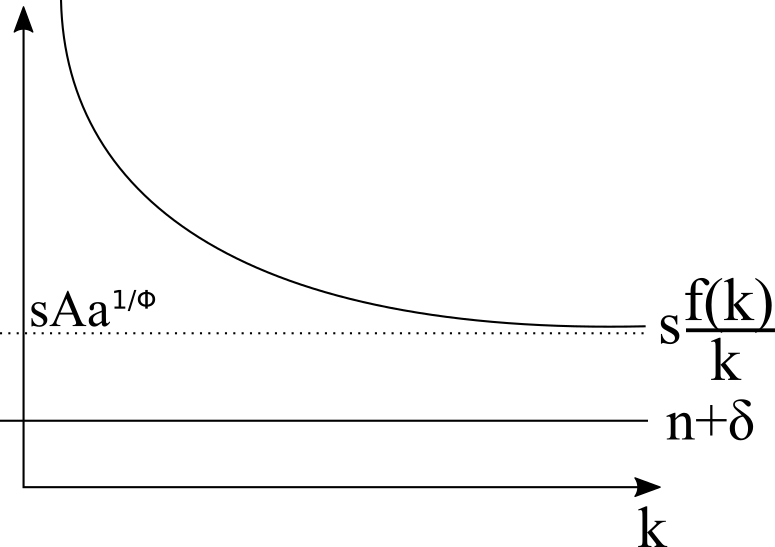
\includegraphics[width=0.5\textwidth]{2f-b}

In this version, there is no single crossing point because $\frac{sf(k)}{k}$ asymptotically approaches $sAa^\invphi$ and never crosses $n+\delta$. Thus there is no steady state and capital will continue to accumulate and grow the economy.












%%%%%%%%%%%%%%%%%%%%%%%%%%%%%%%%%%%%%%%%%%%%%%%
%                Problem 3                    %
%%%%%%%%%%%%%%%%%%%%%%%%%%%%%%%%%%%%%%%%%%%%%%%
\newpage
\section*{Problem 3}
\problem{The Harrod-Domar Model}{
    Prior to the development of the Solow model, work on development and growth often used a Leontief production function
    \begin{equation}
        Y = F(K,L) = min(AK, BL),
        \label{eq:F3}
    \end{equation}
    where $A=0$ and $B=0$. As we discussed above, this corresponds to a CES production function with $\phi\to -\infty$. Well-known papers to use this type of production function are Harrod (1939) and Domar (1946). Growth models that use this production function have since usually been referred to as Harrod-Domar models. Harrod and Domar predicted that capitalist economies would suffer from persistent problems of unemployment of either labor or machines. We now explore how this conclusion follows from the production function \eqref{eq:F3}.
    \vspace{1em}

    \begin{enumerate}[label=(\alph*)]
    \item Rewrite the production function \eqref{eq:F3} in terms of per capita output $y$ and capital per capita $k$. Plot the resulting production function as a function of $k$. Also plot the marginal product of capital as a function of $k$.
    \end{enumerate} 
}

\begin{align} 
    \intertext{stuff}
    y&=x
\end{align}

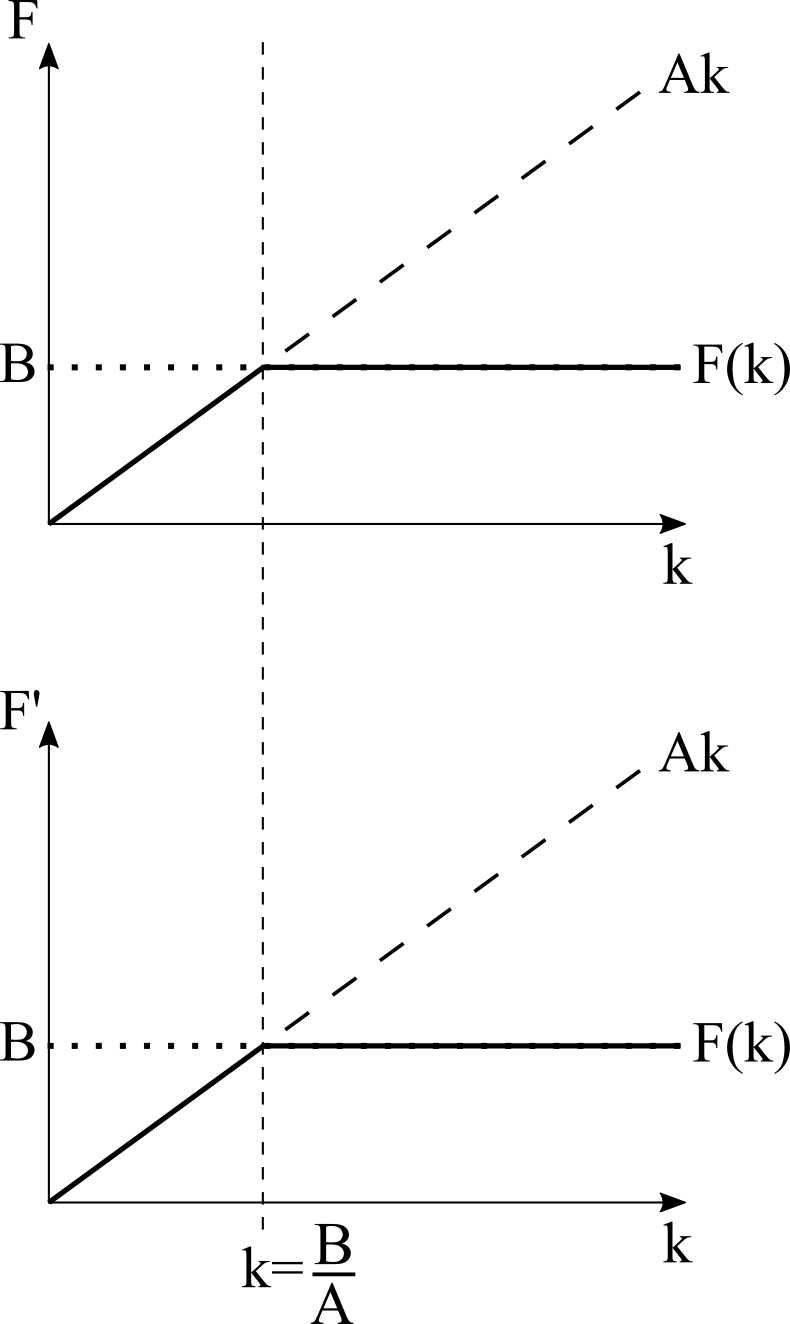
\includegraphics[width=0.5\textwidth]{3a}

%%%%%%%%%%%%%%%%%
%     Part b    %
%%%%%%%%%%%%%%%%%
\newpage\problem{}{
    \begin{enumerate}[label=(\alph*)]
    \setcounter{enumi}{1}
    \item Recall that with a constant savings rate $s$ we have
        \[\frac{\kdot}{k} = \frac{sf(k)}{k} - (n+\delta)\]
    Consider first the case where $sA < (n+\delta)$. Plot $sf(k)/k$ and $n+\delta$ as a function of $k$. Discuss the dynamics of this economy starting from some initial capital stock $k_0$. Comment in particular on the degree of unemployment of labor in the long run in such an economy.
    \end{enumerate} 
}

\begin{align*} 
    \intertext{stuff}
    y&=x
\end{align*}



%%%%%%%%%%%%%%%%%
%     Part c    %
%%%%%%%%%%%%%%%%%
\newpage\problem{}{
    \begin{enumerate}[label=(\alph*)]
    \setcounter{enumi}{2}
    \item Now consider the case were $sA > (n+\delta)$. Again, plot $sf(k)/k$ and $n+\delta$ as a function of $k$. Discuss the dynamics of this economy starting from some initial capital stock $k_0$. Comment on the degree of unemployment of labor in the long run as well as the possible idleness of capital in the long run.
    \end{enumerate} 
}

\begin{align*} 
    \intertext{stuff}
    y&=x
\end{align*}



%%%%%%%%%%%%%%%%%
%     Part d    %
%%%%%%%%%%%%%%%%%
\newpage\problem{}{
    \begin{enumerate}[label=(\alph*)]
    \setcounter{enumi}{3}
    \item Is it possible for both capital and labor to be fully employed in a Harrod-Domar economy in the long run?
    \end{enumerate} 
}
















\end{document}

